\section{Learning from Data}

\begin{wrapfigure}[15]{l}{0.4\linewidth}
    \vspace{-15pt}
    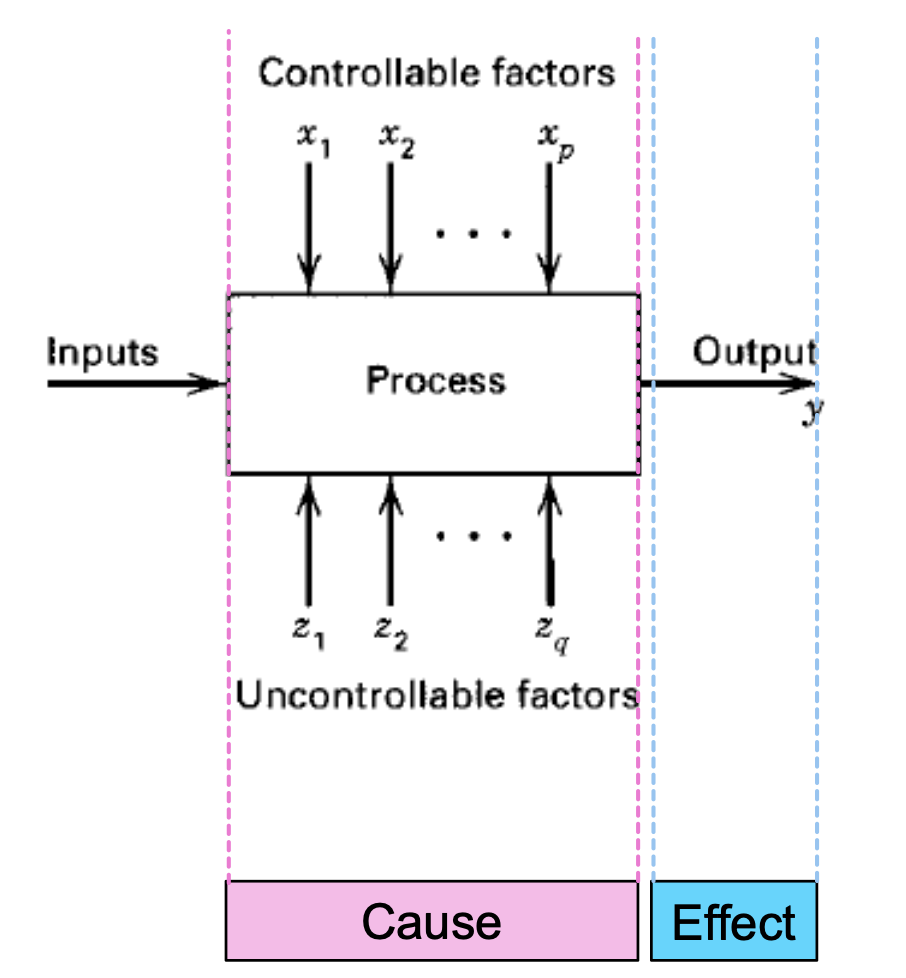
\includegraphics[width=1.15\linewidth]{cause-effect.png}
\end{wrapfigure}

We are in the abstract situation where we have a system with many input variables (\textbf{predictors}) and an output (\textbf{response}). We want to find \textbf{cause-effect relationships}, meaning that when we actively change one of the inputs (\textbf{intervention}), this will cause the output to change. This is what we do in \textbf{experimental studies}. If we can just observe a system under different settings (observational studies), it is much harder to make a statement about causal effects. With observational data, we can typically just make a statement about an association between two variables. One potential danger is the existence of \textbf{confounders} (a common cause for two variables).


\subsection{Experimental Studies}

Before designing an experimental study, we must have a precise research question that is actually testable, i.e., that we can do the appropriate interventions and that we can measure the right response.\medskip

An experimental study consists of:

\begin{itemize}
	\item \textbf{Treatments / Predictors}: the different interventions on the system
	\item \textbf{Experimental units}: the actual objects on which we apply the treatments
	\item A method that assigns experimental units to treatments, typically \textbf{randomization}
	\item \textbf{Response(s)}: the output that we measure
\end{itemize}

\subsubsection{Treatments or Predictors}

We distinguish between the following types of predictors:

\begin{itemize}
	\item Predictors that are of primary interest and that can (ideally) be varied according to our “wishes”
	\item Predictors that are systematically recorded such that potential effects can later be eliminated in our calculations (\textbf{covariates})
	\item Predictors that can be kept constant and whose effects are therefore eliminated
	\item Predictors that we can neither record nor keep constant
\end{itemize}

\subsubsection{Randomization}

Randomization ensures that the only systematic difference between the groups is the treatment. This protects us from confounders and is the reason why a properly randomized experiment allows us to make a statement about a cause-effect relationship between treatment and response. Typically, we do a randomization “within” homogeneous blocks. This restricted version of randomization is called \textbf{blocking}. A block is a subset of experimental units that is more homogeneous than the entire set.

\subsubsection{Experimental and Measurement Units}

An \textbf{experimental unit} is defined as the object on which we apply the treatments by randomization. On the other hand, a \textbf{measurement unit} is the object on which the response is being measured. They do not have to be the same.

\subsubsection{Experimental Error}

Different experimental units will give different responses to the same treatment (\textbf{experimental error}). Therefore we need multiple replicates receiving the same treatment. If the difference between the treatments is much larger than the experimental error, we can conclude that there is a treatment effect.

\subsubsection{Blinding}

\textbf{Blinding} means that those who measure the response do not know which treatment is given. With humans it is common to use \textbf{double-blinding} where in addition the patients do not know the assignment either. Blinding protects us from (unintentional) bias due to expectations.

A \textbf{control treatment} is typically a standard treatment with which we want to compare. It can also be no treatment at all.